\chapter{Quadratura numerica}

	\noindent Un problema classico dell'analisi numerica consiste nell'approssimare integrali definiti di una funzione reale \(f\), definita in un intervallo \((\, a, b \,)\) non per forza limitato, del tipo
	\begin{equation}\label{eq:integrale-con-peso}
		I_w (f) = I_w (f, a, b) = \int_a^b f (x) w (x) \dd{x}
	\end{equation}
	ove \(w \colon (\, a, b \,) \to \R\) è una funzione peso. Questi integrali possono essere approssimati con formule del tipo
	\begin{equation}\label{eq:formula-quadratura}
		I_w (f) \approx S_N (f) = \sum_{i = 1}^N w_i f (x_i)
	\end{equation}
	ove \(w_1, \dots, w_N \in \R\) sono detti \emph{pesi} e \(x_0, \dots, x_N \in \mathcal{I} \supseteq (\, a, b \,)\) sono detti \emph{nodi}. D'ora in avanti supporremo che i nodi \(x_1, \dots, x_N\) siano distinti tra loro e che \(f \in \cont ((\, a, b \,))\) ammetta finito \(I_w (f)\), ovvero sia \(w\)-integrabile.
	
	Se \((\, a, b \,)\) è limitato e \(f \in \cont ([\, a, b \,])\), per l'integrabilità della funzione peso e per il teorema di Weierstrass si ha
	\begin{equation*}
		\abs{\int_a^b f (x) w (x) \dd{x}} \le \int_a^b \abs{f (x)} w (x) \dd{x} \le \norm{f}_\infty \norm{w}_1 < + \infty
	\end{equation*}
	ove si è usata la notazione \(\norm{w}_1 = \int_a^b \abs{w (x)} \dd{x} = \int_a^b w (x) \dd{x}\). Ciò mostra che, in tal caso, \(f\) è \(w\)-integrabile in \((\, a, b \,)\).
	
\section{Formule di Newton-Cotes}
	
	\noindent Indicato con
	\begin{equation*}
		p_{N - 1} (x) = \sum_{i = 1}^N f (x_i) L_i (x)
	\end{equation*}
	il polinomio che interpola le coppie \((x_i, f (x_i))\) per \(i \in \Set{1, \dots, N}\) ove \(L_i\) indica l'\(i\)-esimo polinomio di Lagrange definito nella \eqref{eq:polin-lagrange}, possiamo scrivere
	\begin{equation*}
		\begin{split}
			\int_a^b f (x) w (x) \dd{x} &\approx \int_a^b p_{N - 1} (x) w (x) \dd{x} \\
			&= \int_a^b \sum_{i = 1}^N f (x_i) L_i (x) w (x) \dd{x} \\
			&= \sum_{i = 1}^N \qty(\int_a^b L_i (x) w (x) \dd{x}) f (x_i)
		\end{split}
	\end{equation*}
	Per com'è scritta l'ultima somma, ha senso definire
	\begin{equation*}
		w_i = \int_a^b L_i (x) w (x) \dd{x}
	\end{equation*}
	quali pesi per ogni \(i \in \Set{1, \dots, N}\).
	
	\begin{definizione}[Formula interpolatoria]\label{def:formula-interp}
		Si dice \emph{formula interpolatoria} una formula di quadratura di forma come nella \eqref{eq:formula-quadratura} tale che per ogni \(k \in \Set{1, \dots, N}\) si abbia
		\begin{equation}\label{eq:nodo-formula-interp}
			w_k = \int_a^b L_k (x) w (x) \dd{x}
		\end{equation}
	\end{definizione}

	\begin{definizione}[Grado di precisione]\label{def:grado-precisione}
		Si dice che una formula di quadratura di forma come nella \eqref{eq:formula-quadratura} ha \emph{grado di precisione almeno \(M\)} se è esatta per tutti i polinomi \(p \in \P_M\), ovvero se per ogni \(p \in \P_M\) si verifica
		\begin{equation}\label{eq:grado-precisione}
			\int_a^b p (x) \, w (x) \dd{x} = \sum_{i = 1}^N w_i \, p (x_i)
		\end{equation}
		Si dice, poi, che essa ha \emph{grado di precisione esattamente \(M\)} se ha grado di precisione almeno \(M\) ed esiste \(q \in \P_{M + 1}\) per cui la \eqref{eq:grado-precisione} non sia verificata.
	\end{definizione}

	\begin{teorema}\label{th:interp-grado-precisione}
		Una formula di quadratura definita come nella \eqref{eq:formula-quadratura} è interpolatoria se e solo se ha grado precisione almeno \(N - 1\).
	\end{teorema}

	\begin{proof}
		Mostriamo entrambe le implicazioni.
		
		\begin{description}
			\item[(\(\Rightarrow\))] Per ipotesi sia vera la \eqref{eq:nodo-formula-interp}; se \(f = p_{N - 1} \in \P_{N - 1}\), allora
			\begin{equation*}
				p_{N - 1} (x) = \sum_{i = 1}^N p_{N - 1} (x_i) L_i (x)
			\end{equation*}
			per ogni \(x \in (\, a, b \,)\) e, quindi,
			\begin{equation*}
				\begin{split}
					\int_a^b p_{N - 1} (x) w (x) \dd{x} &= \int_a^b \sum_{i = 1}^N p_{N - 1} (x_i) L_i (x) w (x) \dd{x} \\
					&= \sum_{i = 1}^N p_{N - 1} (x_i) \int_a^b L_i (x) w (x) \dd{x} \\
					&= \sum_{i = 1}^N w_i \, p_{N - 1} (x_i)
				\end{split}
			\end{equation*}
			il che mostra che la formula ha grado di precisione almeno \(N - 1\).
			\item[(\(\Leftarrow\))] Se la formula di quadratura è esatta per tutti i polinomi di grado \(N - 1\), lo è anche per i polinomi di Lagrange di tale grado. Dato che \(L_k (x_i) = \delta_{k, i}\), si ha per ogni \(k \in \Set{1, \dots, N}\)
			\begin{equation*}
				\int_a^b L_k (x) w (x) \dd{x} = \sum_{i = 1}^N w_i L_k (x_i) = \sum_{i = 1}^N w_i \delta_{k, i} = w_k
			\end{equation*}
			Ciò prova che la formula è interpolatoria.\qedhere
		\end{description}
	\end{proof}

	\begin{definizione}[Formule di Newton-Cotes chiuse]
		Dato un intervallo chiuso e limitato \([\, a, b \,] \subseteq \R\), una formula di quadratura definita come nella \eqref{eq:formula-quadratura} si dice \emph{di Newton-Cotes chiusa} se i nodi sono equispaziati, ovvero
		\begin{subequations}
			\begin{equation}
				x_i = a + \frac{(i - 1) (b - a)}{N - 1}
			\end{equation}
		al variare di \(i \in \Set{1, \dots, N}\), e i pesi sono definiti come
			\begin{equation}
				w_i = \int_a^b L_i (x) \dd{x}
			\end{equation}
		al variare di \(i \in \Set{1, \dots, N}\). Una tale formula è interpolatoria e ha grado di precisione almeno \(N - 1\).
		\end{subequations}
	\end{definizione}

	\begin{figure}[tpb]
		\centering
		
		\begin{tikzpicture}
			\begin{axis}[no marks, domain = 0:3, xmax = 3.14, ymax = 1.15, axis lines = center]
				\addplot+[smooth, black] {sin(deg(x))};
				\filldraw[fill = red, draw = red, fill opacity = 0.2] (0.5,0) -- (0.5, \drawsinlua{0.5}) -- (2, \drawsinlua{2}) -- (2,0) -- cycle;
				\filldraw[fill = blue, draw = blue, fill opacity = 0.1] (0.5, 0) -- (0.5, \drawsinlua{0.5}) to[parabola through={(1.25, \drawsinlua{1.25})}] (2, \drawsinlua{2}) -- (2,0) -- cycle;
			\end{axis}
		\end{tikzpicture}
		\caption{Confronto tra la regola del trapezio (in rosso) e la regola di Cavalieri-Simpson (in blu) per l'approssimazione di \(\int_{1 / 2}^2 \sin x \dd{x}\).}
	\end{figure}

	Vediamo ora alcuni casi particolari di formule di Newton-Cotes chiuse.
	
	\begin{definizione}[Regola del trapezio]\label{def:regola-trapezio}
		Si chiama \emph{regola del trapezio} la formula di quadratura
		\begin{equation}\label{eq:regola-trapezio}
			S_2 (f) = S_2 (f, a, b) = \frac{b - a}{2} \qty(f (a) + f (b))
		\end{equation}
	\end{definizione}

	Si può dimostrare che, posto \(h = b - a\), l'errore compiuto dalla formula in \eqref{eq:regola-trapezio} è pari a
	\begin{equation}\label{eq:regola-trapezio-errore}
		\mathcal{E}_2 (f) = I (f) - S_2 (f) = - \frac{h^3}{12} f'' (\xi)
	\end{equation}
	per un certo \(\xi \in (\, a, b \,)\), se si suppone che \(f\) sia derivabile due volte in \((\, a, b \,)\). Dalla \eqref{eq:regola-trapezio-errore} risulta evidente che \(S_2\) ha grado di precisione esattamente \(1\), perché
	\begin{equation*}
		f \in \P_1 \implies \forall \xi \in (\, a, b \,) \colon f'' (\xi) = 0 \implies \mathcal{E}_2 (f) = 0
	\end{equation*}
	mentre
	\begin{multline*}
		f \in \P_2 \setminus \P_1 \implies
		\begin{cases*}
			f (x) = a x^2 + b x + c \\
			a \ne 0
		\end{cases*} \\
		\implies \forall \xi \in (\, a, b \,) \colon f'' (\xi) = 2 a \ne 0 \implies \mathcal{E}_2 (f) \ne 0
	\end{multline*}

	\begin{osservazione}
		Posti \(x_1 = a\) e \(x_2 = b\), si ha
		\begin{align*}
			L_1 (x) &= \frac{x - b}{a - b} &
			L_2 (x) &= \frac{x - a}{b - a}
		\end{align*}
		e, visto che \(w \equiv 1\), si ottiene
		\begin{equation*}
			\begin{split}
				w_1 &= \int_a^b L_1 (x) \dd{x} = \int_a^b \frac{x - b}{a - b} \dd{x} \\
				&= \frac{1}{a - b} \int_a^b (x - b) \dd{x} = \frac{1}{a - b} \eval[\frac{(x - b)^2}{2}|_a^b \\
				&= \frac{1}{\cancel{a - b}} \frac{- (a - b)^{\cancel{2}}}{2} = \frac{b - a}{2}
			\end{split}
		\end{equation*}
		e
		\begin{equation*}
			\begin{split}
				w_2 &= \int_a^b L_2 (x) \dd{x} = \int_a^b \frac{x - a}{b - a} \dd{x} \\
				&= \frac{1}{b - a} \int_a^b (x - a) \dd{x} = \frac{1}{b - a} \eval[\frac{(x - a)^2}{2}|_a^b \\
				&= \frac{1}{\cancel{b - a}} \frac{(b - a)^{\cancel{2}}}{2} = \frac{b - a}{2}
			\end{split}
		\end{equation*}
		ovvero che la regola del trapezio è davvero una formula interpolatoria.
	\end{osservazione}

	\begin{definizione}[Regola di Cavalieri-Simpson]\label{def:regola-cavalieri}
		Si chiama \emph{regola di Cavalieri-Simpson} la formula di quadratura
		\begin{equation}\label{eq:regola-cavalieri}
			S_3 (f) = S_3 (f, a, b) = \frac{b - a}{6} \qty[f (a) + 4 f \qty(\frac{a + b}{2}) + f (b)]
		\end{equation}
	\end{definizione}

	Si può dimostrare che l'errore compiuto dalla formula in \eqref{eq:regola-cavalieri}, posto \(h = (b - a) / 2\), è
	\begin{equation}\label{eq:regola-cavalieri-errore}
		\mathcal{E}_3 (f) = I (f) - S_3 (f) = - \frac{h^5}{90} f^{(4)} (\xi)
	\end{equation}
	per un certo \(\xi \in (\, a, b \,)\), se si suppone che \(f\) sia derivabile quattro volte in \((\, a, b \,)\). Il grado di precisione di questa formula è esattamente \(3\), perché dalla \eqref{eq:regola-cavalieri-errore} segue che
	\begin{equation*}
		f \in \P_3 \implies \forall \xi \in (\, a, b \,) \colon f^{(4)} (\xi) = 0 \implies \mathcal{E}_3 (f) = 0
	\end{equation*}
	mentre
	\begin{multline*}
		f \in \P_4 \setminus \P_3 \implies
		\begin{cases*}
			f (x) = a x^4 + b x^3 + c x^2 + d x + e \\
			a \ne 0
		\end{cases*} \\
		\implies \forall \xi \in (\, a, b \,) \colon f^{(4)} (\xi) = 24 a \ne 0 \implies \mathcal{E}_3 (f) \ne 0
	\end{multline*}

	\begin{osservazione}
		Posti \(x_1 = a\), \(x_2 = (a + b) / 2\) e \(x_3 = b\), si ha
		\begin{align*}
			L_1 (x) &= \frac{(2 x - a - b) (x - b)}{(a - b)^2} \\
			L_2 (x) &= - 4 \frac{(x - a) (x - b)}{(a - b)^2} \\
			L_3 (x) &= \frac{(2 x - a - b)}{(b - a)^2}
		\end{align*}
		e, visto che \(w \equiv 1\), si ottiene
		\begin{equation*}
			\begin{split}
				w_1 &= \int_a^b L_1 (x) \dd{x} = \frac{1}{(a - b)^2} \int_a^b (2 x - a - b) (x - b) \dd{x} \\
				&= \frac{1}{(a - b)^2} \qty(\eval[(x^2 - a x - b x) (x - b)|_a^b - \eval[\frac{x^3}{3} - \frac{a x^2}{2} - \frac{b x^2}{2}|_a^b) \\
				&= \frac{1}{(a - b)^2} \qty(\frac{b^3}{6} - \frac{a b^2}{2} + \frac{a^2 b}{2} - \frac{a^3}{6}) \\
				&= \frac{(b - a)^3}{6 (a - b)^2} = \frac{b - a}{6}
			\end{split}
		\end{equation*}
		e
		\begin{equation*}
			\begin{split}
				w_2 &= \int_a^b L_2 (x) \dd{x} = - \frac{4}{(a - b)^2} \int_a^b (x - a) (x - b) \dd{x} \\
				&= - \frac{4}{(a - b)^2} \eval[\frac{x^3}{3} - \frac{a + b}{2} x^2 + a b x|_a^b \\
				&= - \frac{4}{(a - b)^2} \qty(\frac{a^3}{6} - \frac{a^2 b}{2} + \frac{a b^2}{2} - \frac{b^3}{6}) \\
				&= -\frac{4 (a - b)^3}{6 (a - b)^2} = \frac{2}{3} (b - a)
			\end{split}
		\end{equation*}
		e infine
		\begin{equation*}
			\begin{split}
				w_3 &= \int_a^b L_3 (x) \dd{x} = \frac{1}{(b - a)^2} \int_a^b (2 x - a - b) (x - a) \dd{x} \\
				&= \frac{1}{(b - a)^2} \qty(\eval[(x^2 - a x - b x) (x - a)|_a^b - \eval[\frac{x^3}{3} - \frac{a x^2}{2} - \frac{b x^2}{2}|_a^b) \\
				&= \frac{1}{(b - a)^2} \qty(\frac{a^3}{6} - \frac{a^2 b}{2} + \frac{a b^2}{2} - \frac{b^3}{6}) \\
				&= \frac{(b - a)^3}{6 (b - a)^2} = \frac{b - a}{6}
			\end{split}
		\end{equation*}
		ovvero che la regola di Cavalieri-Simpson risulta essere davvero una formula interpolatoria.
	\end{osservazione}

	Sia per la regola del trapezio che per quella di Cavalieri-Simpson si ricorre a stime che fanno uso del nucleo di Peano qualora le funzioni in esame non siano derivabili un numero sufficiente di volte a rendere ben definite la \eqref{eq:regola-trapezio-errore} e la \eqref{eq:regola-cavalieri-errore}.
	
	Ricordiamo, poi, che per \(N \ge 8\) le formule di Newton-Cotes chiuse hanno pesi di segno discorde; ciò le rende instabili per quanto riguarda la propagazione degli errori.
	
	Riportiamo altre formule di Newton-Cotes di grado superiore a \(2\), usando la notazione \(f_k = f (x_k)\) e ponendo \(h = (b - a) / (N - 1)\), ove \(N\) è il numero dei nodi:
		\begin{subequations}
			\begin{itemize}
				\item la formula dei tre ottavi
				\begin{equation}
					\frac{3h}{8} (f_1 + 3 f_2 + 3 f_3 + f_4)
				\end{equation}
				\item la regola di Milne-Boole
				\begin{equation}
					\frac{2 h}{45} (7 f_1 + 32 f_2 + 12 f_3 + 32 f_4 + 7 f_5)
				\end{equation}
				\item la formula a sei punti
				\begin{equation}
					\frac{5 h}{288} (19 f_1 + 75 f_2 + 50 f_3 + 50 f_4 + 75 f_5 + 19 f_6)
				\end{equation}
				\item la regola di Weedle-Hardy
				\begin{equation}
					\frac{h}{140} (41 f_1 + 216 f_2 + 27 f_3 + 272 f_4 + 27 f_5 + 216 f_6 + 41 f_7)
				\end{equation}
				\item la formula a otto punti
				\begin{multline}
					\frac{7 h}{17280} (751 f_1 + 3577 f_2 + 1323 f_3 + 2989 f_4 \\
					+ 2989 f_5 + 1323 f_6 + 3577 f_7 + 751 f_8)
				\end{multline}
				\item la formula a nove punti
				\begin{multline}
					\frac{4 h}{14175} (989 f_1 + 5888 f_2 - 928 f_3 + 10496 f_4 \\
					- 4540 f_5 + 10496 f_6 - 928 f_7 + 5888 f_8 + 989 f_9)
				\end{multline}
				\item la formula a dieci punti
				\begin{multline}
					\frac{9 h}{89600} (2857 f_1 + 15741 f_2 + 1080 f_3 + 19344 f_4 + 5788 f_5 \\
					+ 5788 f_6 + 19344 f_7 + 1080 f_8 + 15741 f_9 + 2857 f_{10})
				\end{multline}
				\item la formula a undici punti
				\begin{multline}
					\frac{5 h}{\num{2999376}} (16067 f_1 + 106300 f_2 - 48525 f_3 \\
					+ 272400 f_4 - 260550 f_5 + 427368 f_6 - 260550 f_7 \\
					+ 272400 f_8 - 48525 f_9 + 106300 f_{10} + 16067 f_{11})
				\end{multline}
			\end{itemize}
		\end{subequations}
	
\section{Formule di Newton-Cotes composte}
	
	\noindent Dato che le formule di Newton-Cotes sono generalmente instabili per \(N \ge 8\), è necessario trovare formule di quadratura che facciano uso di altrettanti nodi ma che siano numericamente stabili.
	
	\begin{definizione}[Formule di Newton-Cotes composte]
		Suddiviso l'intervallo \([\, a, b \,]\) in \(N\) subintervalli \(T_j = [\, x_j, x_{j + 1} \,]\) tali che \(x_j = a + j h_N\), ove si è posto \(h_N = (b - a) / N\), si dice \emph{formula di Newton-Cotes composta} una formula di quadratura del tipo
		\begin{equation}\label{eq:formule-composte}
			I (f) \approx \sum_{j = 0}^{N - 1} S (f, x_j, x_{j + 1})
		\end{equation}
		ove \(S\) è una formula di Newton-Cotes chiusa.
	\end{definizione}

	Questa definizione segue dalle proprietà dell'integrale:
	\begin{equation*}
		\int_a^b f (x) \dd{x} = \sum_{j = 0}^{N - 1} \int_{x_j}^{x_{j + 1}} f (x) \dd{x} \approx \sum_{j = 0}^{N - 1} S (f, x_j, x_{j + 1})
	\end{equation*}

	\begin{figure}[tpb]
		\centering
		
		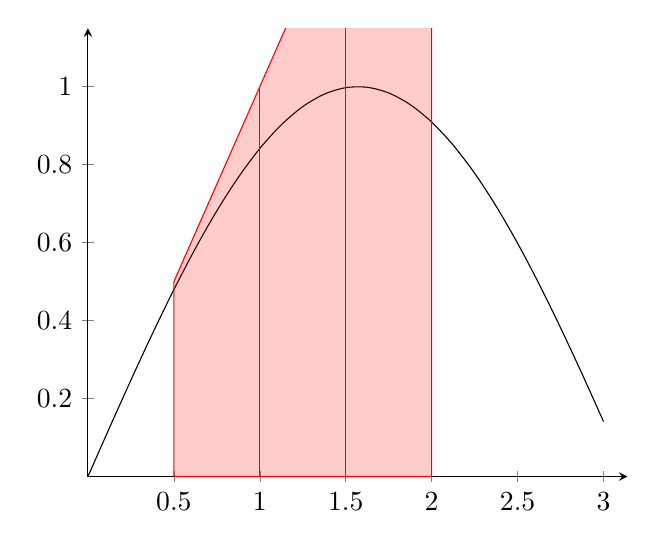
\begin{tikzpicture}
			\begin{axis}[no marks, domain = 0:3, xmax = 3.14, ymax = 1.15, axis lines = center]
				\addplot+[smooth, black] {sin(deg(x))};
				\filldraw[fill = red, draw = red, fill opacity = 0.2] (0.5,0) -- (0.5, \drawsinlua{0.5}) -- (1, \drawsinlua{1}) -- (1.5, \drawsinlua{1.5}) -- (2, \drawsinlua{2}) -- (2,0) -- cycle;
				\draw[red] (1, \drawsinlua{1}) -- (1,0) (1.5, \drawsinlua{1.5}) -- (1.5,0);
			\end{axis}
		\end{tikzpicture}
		\caption{Rappresentazione dell'approssimazione di \(\int_{1 / 2}^2 \sin x \dd{x}\) tramite la regola dei trapezi.}
	\end{figure}

	Vediamo ora delle formule di Newton-Cotes composte particolari.
	
	\begin{definizione}[Formula dei trapezi]
		Si chiama \emph{formula dei trapezi} o \emph{del trapezio composta} la formula di quadratura su \([\, a, b \,]\)
		\begin{equation}\label{eq:formula-trapezi}
			S_2^{(c)} (f, N) = \frac{b - a}{N} \qty[\frac{f (x_0)}{2} + f (x_1) + \dots + f (x_{N - 1}) + \frac{f (x_N)}{2}]
		\end{equation}
		ove \(x_i = a + i h_N\) per \(i \in \Set{0, \dots, N}\).
	\end{definizione}

	Si può dimostrare che, se \(f\) è derivabile due volte in \((\, a, b \,)\), l'errore commesso dalla \eqref{eq:formula-trapezi} è pari a
	\begin{equation}\label{eq:formula-trapezi-errore}
		\mathcal{E}_2^{(c)} (f) = I (f) - S_2^{(c)} (f, N) = - \frac{b - a}{12} h_N^2 f'' (\xi)
	\end{equation}
	per un certo \(\xi \in (\, a, b \,)\). Il grado di precisione di questa formula è ancora \(1\), ma per \(N \ge 1\) si ha \(h_N \le h\), da cui segue che \(\abs{\mathcal{E}_2^{(c)} (f)} \le \abs{\mathcal{E}_2 (f)}\).
	
	Sotto ipotesi piú stringenti è possibile migliorare la stima dell'andamento dell'errore \(\mathcal{E}_2^{(c)} (f)\), che in base alla \eqref{eq:formula-trapezi-errore} è \(\order{1 / N^2}\).
	
	\begin{teorema}[Formula di Eulero-Maclaurin]
		Se \(f \in \cont^{2 M + 2} ([\, a, b \,])\), allora esiste \(\xi \in (\, a, b \,)\) tale che
		\begin{multline}\label{eq:formula-eulero-maclaurin}
			\int_a^b f (x) \dd{x} = S_2^{(c)} (f, N) - \qty[\sum_{k = 1}^M \frac{B_{2 k}}{(2 k)!} h_N^{2 k} \qty(f^{(2 k - 1)} (b) - f^{(2 k - 1)}) (a)] \\
			- \frac{B_{2 M + 2}}{(2 M + 2)!} h_N^{2 M + 2} (b - a) f^{(2 M + 2)} (\xi)
		\end{multline}
		ove i \(B_k\) sono i numeri di Bernoulli.
	\end{teorema}

	Se ci poniamo nel caso particolare in cui \(f^{(2 k -1)} (a) = f^{(2 k - 1)} (b)\) per ogni \(k \in \Set{1, \dots, M}\), la sommatoria nella \eqref{eq:formula-eulero-maclaurin} si annulla e diviene evidente che \(\mathcal{E}_2^{(c)} (f)\) è in tal caso \(\order{1 / N^{2 M + 2}}\). In casi ancor piú specifici, l'errore decresce esponenzialmente.
	
	\begin{teorema}
		Se \(f \colon [\, 0, 2 \pi \,] \to \R\) è una funzione analitica e periodica di periodo \(2 \pi\) tale che esistano \(a, M > 0\) tali che \(\abs{f (z)} \le M\) per ogni \(z \in \C\) tale che \(\Im z > - a\), allora per ogni \(N \in \N^*\) \(f\) verifica
		\begin{equation}
			\abs{S_2^{(c)} (f, N) - I (f)} \le \frac{2 \pi M}{\ee^{a N} - 1}
		\end{equation}
		e la costante \(2 \pi\) è la minima costante che renda vera tale diseguaglianza.
	\end{teorema}

	\begin{definizione}[Formula di Cavalieri-Simpson composta]
		Si chiama \emph{formula di Cavalieri-Simpson composta} la formula di quadratura su \([\, a, b \,]\)
		\begin{equation}\label{eq:formula-simpson-composta}
			S_3^{(c)} (f, N) = \frac{h_N}{6} \qty[f (x_0) + 2 \sum_{r = 1}^{N - 1} f (x_{2 r}) + 4 \sum_{s = 0}^{N - 1} f (x_{2 s + 1}) + f (x_{2 N})]
		\end{equation}
		ove \(x_k = a + k h_N / 2\) per \(k \in \Set{0, \dots, 2 N}\).
	\end{definizione}

	Si può dimostrare che, se \(f\) è derivabile quattro volte in \((\, a, b \,)\), l'errore compiuto dalla \eqref{eq:formula-simpson-composta} è
	\begin{equation}
		\mathcal{E}_3^{(c)} (f) = I (f) - S_3^{(c)} (f, N) = - \frac{b - a}{180} \qty(\frac{h_N}{2})^4 f^{(4)} (\xi)
	\end{equation}
	per un certo \(\xi \in (\, a, b \,)\). Il grado di precisione di questa formula è esattamente \(3\), ma, analogamente alla regola dei trapezi composta, si ha che \(\abs{\mathcal{E}_3^{(c)} (f)} \le \abs{\mathcal{E}_3 (f)}\) perché \(h_N \le h\).
	
	\begin{figure}[tpb]
		\centering
		
		\begin{tikzpicture}
			\begin{axis}[no marks, domain = 0:3, xmax = 3.14, ymax = 1.15, axis lines = center]
				\addplot+[smooth, black, samples = 350] {sin(deg(x))};
				\filldraw[fill = blue, draw = blue, fill opacity = 0.1] (0.5,0) -- (0.5, \drawsinlua{0.5}) to[parabola through={(0.875, \drawsinlua{0.875})}] (1.25, \drawsinlua{1.25}) to[parabola through={(1.625, \drawsinlua{1.625})}] (2,\drawsinlua{2}) -- (2,0) -- cycle;
				\draw[densely dashed, blue] (0.875, 0) -- (0.875, \drawsinlua{0.875}) (1.625, 0) -- (1.625, \drawsinlua{1.625});
				\draw[blue] (1.25, \drawsinlua{1.25}) -- (1.25,0);
			\end{axis}
		\end{tikzpicture}
		\caption{Rappresentazione dell'approssimazione di \(\int_{1 / 2}^2 \sin x \dd{x}\) tramite la regola di Cavalieri-Simpson composta.}
	\end{figure}
	
\section{Formule gaussiane}
	
	\noindent Le formule interpolatorie di Newton-Cotes presuppongono sempre che i nodi in esame siano equispaziati e hanno grado di precisione almeno \(N - 1\), ove \(N\) è il numero dei nodi, benché le formule con un numero dispari di nodi come quella di Cavalieri-Simpson abbiano grado di precisione esattamente \(N\).
	
	Vogliamo ora studiare formule che si possano applicare anche per integrali su intervalli \((\, a, b \,)\) non necessariamente limitati e valide per funzioni peso diverse da \(w \equiv 1\); vogliamo, poi, trovare formule che abbiano un grado di precisione piú alto a parità di nodi.
	
	Il problema di dover calcolare un integrale di una funzione \(f \colon (\, a, b \,) \to \R\) come nella \eqref{eq:integrale-con-peso} è di gran lunga piú generale rispetto all'integrazione di una funzione continua su un intervallo chiuso e limitato: l'integranda \(f w\), infatti, potrebbe non essere continua in \([\, a, b \,]\), come ad esempio accade usando la funzione peso di Chebyshev, discontinua in \(\pm 1\); l'intervallo, poi, potrebbe non essere nemmeno limitato, come accade quando si usa la funzione peso di Laguerre o quella di Hermite.
	
	\begin{teorema}\label{th:formula-gaussiana-esiste-unica}
		Data una funzione peso \(w \colon (\, a, b \,) \to \R\), per ogni \(n \in \N^*\) esistono un'unica \(n\)-upla \(x_1, \dots, x_n\) di nodi e un'unica \(n\)-upla di pesi \(w_1, \dots, w_n\) tali che la formula di quadratura per approssimare \(I_w (f)\) che ha questi come nodi e come pesi abbia grado di precisione almeno \(2 n - 1\). Tali nodi sono gli zeri del polinomio ortogonale rispetto a \(w\) di grado \(n\) \(\varphi_n (x) = A_n (x - x_1) \cdots (x - x_n)\), mentre i pesi sono individuati per ogni \(i \in \Set{1, \dots, n}\) da
		\begin{equation}\label{eq:formule-gauss-pesi}
			w_i = \int_a^b L_i (x) w (x) \dd{x} = \int_a^b L_i^2 (x) w (x) \dd{x}
		\end{equation}
	\end{teorema}

	\begin{proof}
		Dimostriamo innanzitutto che una formula di quadratura cosí definita ha grado di precisione almeno \(2 n - 1\). Siano dunque \(p_{2 n - 1} \in \P_{2 n - 1}\) e \(q_{n - 1}, r_{n - 1} \in \P_{n - 1}\) tali che
		\begin{equation*}
			p_{2 n - 1} = q_{n - 1} \varphi_n + r_{n - 1}
		\end{equation*}
		Poiché \(\varphi_n\) è il polinomio ortogonale rispetto a \(w\) di grado \(n\), si ha
		\begin{multline*}
			\int_a^b q_{n - 1} (x) \varphi_n (x) w (x) \dd{x} = (q_{n - 1}, \varphi_n)_{2, w} \\
			= \qty(\sum_{j = 0}^{n - 1} \gamma_j \varphi_j, \varphi_n)_{2, w} = \sum_{j = 0}^{n - 1} \gamma_j (\varphi_j, \varphi_n)_{2, w} = 0
		\end{multline*}
		Dalla \eqref{eq:formule-gauss-pesi} è evidente che la formula di quadratura definita è interpolatoria e, quindi, esatta su ogni polinomio di grado \(n - 1\), in quanto basata su \(n\) punti a due a due distinti. Dato che, per ogni zero \(x_k\) di \(\varphi_n\) si ha
		\begin{equation*}
			p_{2 n - 1} (x_k) = q_{n - 1} (x_k) \varphi_n (x_k) + r_{n - 1} (x_k) = r_{n - 1} (x_k)
		\end{equation*}
		segue che
		\begin{equation*}
			\begin{split}
				\int_a^b p_{2 n - 1} (x) w (x) \dd{x} &= \cancel{\int_a^b q_{n - 1} (x) \varphi_n (x) w (x) \dd{x}} + \int_a^b r_{n - 1} (x) w (x) \dd{x} \\
				&= \int_a^b r_{n - 1} (x) w (x) \dd{x} = \sum_{k = 1}^n w_k \, r_{n - 1} (x_k) \\
				&= \sum_{k = 1}^n w_k \, p_{2 n - 1} (x_k)
			\end{split}
		\end{equation*}
		ovvero che la formula di quadratura ha grado di precisione almeno \(2 n - 1\).
		
		Visto che \(\deg L_i^2 = 2 (n - 1) < 2 n - 1\) per ogni \(i \in \Set{1, \dots, n}\), la formula di quadratura in esame integra esattamente i quadrati dei polinomi di Lagrange; da ciò segue che per ogni \(i \in \Set{1, \dots, n}\)
		\begin{equation*}
			0 < \int_a^b L_i^2 (x) w (x) \dd{x} = \sum_{k = 1}^n w_k L_i^2 (x_k) = \sum_{k = 1}^n w_k \delta_{k, i} = w_i
		\end{equation*}
	
		Supponiamo ora che esista un'altra formula interpolatoria con grado di precisione almeno \(2 n - 1\) che abbia nodi \(\tilde{x}_1, \dots, \tilde{x}_n\) e pesi \(\tilde{w}_1, \dots, \tilde{w}_n\). Per quanto visto sopra, dal grado di precisione della formula segue che \(\tilde{w}_j > 0\) per ogni \(j \in \Set{1, \dots, n}\). A meno di cambiare gli indici, possiamo supporre che sia i nodi \(x_j\) sia i nodi \(\tilde{x}_j\) abbiano ordine crescente. Indicato con \(\tilde{L}_j\) il \(j\)-esimo polinomio di Lagrange per i nodi \(\tilde{x}_j\), che ha grado \(n - 1\), si ha
		\begin{multline*}
				0 = \qty(\tilde{L}_j, \varphi_n)_{2, w} = \int_a^b \tilde{L}_j (x) \varphi_n (x) w (x) \dd{x} \\
				= \sum_{k = 1}^n \tilde{w}_k \tilde{L}_j (\tilde{x}_k) \varphi_n (\tilde{x}_k) = \tilde{w}_j \varphi_n (\tilde{x}_j)
		\end{multline*}
		e, dato che \(\tilde{w}_j > 0\) per ogni \(j\), risulta che \(\tilde{x}_j\) è uno zero di \(\varphi_n\). Ciò prova che i \(\tilde{x}_j\) sono al piú \(n\), ma potrebbero essere meno. Per assurdo siano in numero \(m < n\): potremmo costruire il polinomio di grado \(m\)
		\begin{equation*}
			p_m (x) = \prod_{j = 1}^m \qty(x - \tilde{x}_j) \ne 0
		\end{equation*}
		che, elevato al quadrato, avrebbe grado \(2 m \le 2 (n - 1) = 2 n - 2\) e, quindi,
		\begin{equation*}
			0 < \int_a^b p_m^2 (x) w (x) \dd{x} = \sum_{j = 1}^m \tilde{w}_j \prod_{k = 1}^m \qty(\tilde{x}_j - \tilde{x}_k)^2 = 0
		\end{equation*}
		che è assurdo. Da ciò si ottiene che i nodi \(\tilde{x}_j\) sono esattamente \(n\), ovvero \(x_j = \tilde{x}_j\) per ogni \(j \in \Set{1, \dots, n}\) e, dato che \(L_j = \tilde{L}_j\), si conclude anche che \(w_j = \tilde{w}_j\) per ogni \(j\).
	\end{proof}

	\begin{osservazione}
		Una formula gaussiana a \(n\) nodi non può avere grado di precisione superiore a \(2 n - 1\). Posto, infatti, \(p_n (x) = \prod_{j = 1}^n (x - x_j) \ne 0\), il polinomio \(p_n^2 (x)\) avrebbe grado \(2 n\) e, quindi,
		\begin{equation*}
			0 < \int_a^b p_n^2 (x) w (x) \dd{x} = \sum_{j = 1}^n w_j \prod_{k = 1}^n (x_j - x_k)^2 = 0
		\end{equation*}
		che è assurdo.
	\end{osservazione}

\section[Stabilità delle formule]{Stabilità di una formula di quadratura}
	
	\begin{teorema}
		Indichiamo con \(I_n (f) = \sum_{i = 1}^n w_{i, n} f (x_{i, n})\) la regola di Newton-Cotes a \(n\) nodi su \([\, a, b \,]\) e poniamo \(h = (b - a) / (n - 1)\). Se \(n\) è dispari e \(f \in \cont^{n + 1} ([\, a, b \,])\), allora esiste \(\eta \in (\, a, b \,)\) tale che
		\begin{subequations}
			\begin{equation}
				I (f) - I_n (f) = C_n h^{n + 2} f^{(n + 1)} (\eta)
			\end{equation}
			ove
			\begin{equation}
				C_n = \frac{1}{(n + 1)!} \int_0^n \mu^2 (\mu - 1) \cdots (\mu - n - 1) \dd{\mu}
			\end{equation}
		\end{subequations}
		Se \(n\) è pari e \(f \in \cont^{n} ([\, a, b \,])\), allora esiste \(\eta \in (\, a, b \,)\) tale che
		\begin{subequations}
			\begin{equation}
				I (f) - I_n (f) = C_n h^{n + 1} f^{(n)} (\eta)
			\end{equation}
			ove
			\begin{equation}
				C_n = \frac{1}{n!} \int_0^{n - 1} \mu (\mu - 1) \cdots (\mu - n - 1) \dd{\mu}
			\end{equation}
		\end{subequations}
	\end{teorema}

	Questo risultato generale conferma quanto trovato nella \eqref{eq:regola-trapezio-errore} e nella \eqref{eq:regola-cavalieri-errore}.
	
	\begin{teorema}
		Chiamata \(I_n (f)\) la formula gaussiana a \(n\) nodi relativa all'integrale \(I_w (f)\) con funzione peso \(w\) sull'intervallo limitato \((\, a, b \,)\), se \(f \in \cont^{2 n} ((\, a, b \,))\), allora esiste \(\eta \in (\, a, b \,)\) tale che
		\begin{equation}
			I_w (f) - I_n (f) = \frac{\gamma_n}{A_n^2 (2 n)!} f^{(2 n)} (\eta)
		\end{equation}
		ove \(A_n\) è il coefficiente di grado \(n\) del polinomio ortogonale \(\varphi_n\) rispetto a \(w\) e \(\gamma_n = \int_a^b \varphi_n^2 (x) w (x) \dd{x}\).
	\end{teorema}

	\begin{figure}[tpb]
		\centering
		
		\begin{tikzpicture}
			\begin{axis}[ymode=log, only marks, legend entries = {Newton-Cotes, Gauss-Legendre}, legend pos = north east, xtick = {0, 5, ..., 35}]
				\addplot table {risorse/newcot.dat};
				\addplot table {risorse/errgauss.dat};
			\end{axis}
		\end{tikzpicture}
		
		\caption{Confronto tra i fattori di errore indipendenti da \(f\) relativi alle formule di Newton-Cotes e alle formule di Gauss-Legendre.}\label{fig:legendre-newton}
	\end{figure}

	In particolare, se \(w \equiv 1\) sull'intervallo \((\, -1, 1 \,)\), allora l'errore commesso dalla formula di Gauss-Legendre è pari a
	\begin{equation*}
		\mathcal{E}_n (f) = I (f) - I_n (f) = \frac{2^{2 n + 1} (n!)^4}{(2 n + 1) [(2 n)!]^3} f^{(2 n)} (\eta) \qquad \exists \eta \in (\, -1, 1 \,)
	\end{equation*}
	Nella Figura~\ref{fig:legendre-newton} è evidente che il fattore di \(\mathcal{E}_n (f)\) indipendente da \(f\) abbia una decrescita di gran lunga piú veloce rispetto all'errore commesso con le formule di Newton-Cotes chiuse.
	
	Considerata una funzione peso \(w\) sull'intervallo generalizzato \((\, a, b \,)\), supponiamo di avere una formula di quadratura \(S_n\) tale che
	\begin{equation*}
		I_w (f) \approx S_n (f) = \sum_{j = 1}^n w_j f_j
	\end{equation*}
	ove \(f_j = f (x_j)\) con gli \(x_j\) scelti secondo quanto richiesto da \(f\). In questa sezione vogliamo capire quanto errore si commetta sostituendo gli \(f_j\) con dei valori perturbati \(\tilde{f}_j\), ovvero calcolando
	\begin{equation*}
		I_w (f) \approx \tilde{S}_n (f) = \sum_{j = 1}^n w_j \tilde{f}_j
	\end{equation*}

	Per la disuguaglianza triangolare si ha
	\begin{multline*}
		\abs{S_n (f) - \tilde{S}_n (f)} = \abs{\sum_{j = 1}^n w_i \qty(f_j - \tilde{f}_j)} \\
		\le \sum_{j = 1}^n \abs{w_j} \abs{f_j - \tilde{f}_j} \le \qty(\sum_{j = 1}^n \abs{w_j}) \max_j \abs{f_j - \tilde{f}_j}
	\end{multline*}
	e il termine \(\sum_{j = 1}^n \abs{w_j}\) è l'\emph{indice di stabilità} della formula di quadratura \(S_n\).
	
	Se supponiamo che \(S_n\) abbia grado di precisione almeno \(0\) e individuiamo i pesi positivi \(w_1^+, \dots, w_{n^+}^+\) e negativi \(w_1^-, \dots, w_{n^-}^-\), allora
	\begin{equation*}
		\begin{split}
			\int_a^b w (x) \dd{x} &= \int_a^b 1 \cdot w (x) \dd{x} = \sum_{j = 1}^n w_j = \sum_{j = 1}^{n^+} w_j^+ + \sum_{j = 1}^{n^-} w_j^- \\
			&= \sum_{j = 1}^{n^+} \abs{w_j^+} + \qty(\sum_{j = 1}^{n^-} \abs{w_j^-} - \sum_{j = 1}^{n^+} \abs{w_j^+}) - \sum_{j = 1}^{n^-} \abs{w_j^-} \\
			&= \sum_{j = 1}^n \abs{w_j} - 2 \sum_{k = 1}^{n^-} \abs{w_k^-}
		\end{split}
	\end{equation*}
	da cui segue che
	\begin{equation}
		\sum_{j = 1}^n \abs{w_j} = \int_a^b w (x) \dd{x} + 2 \sum_{k = 1}^{n^-} \abs{w_k^-}
	\end{equation}
	In base a ciò, si può affermare che la presenza di pesi negativi peggiora l'indice di stabilità della formula \(S_n\). Se, invece, \(S_n\) non prevede pesi negativi, allora \(\sum_{j = 1}^n \abs{w_j} = \int_a^b w (x) \dd{x}\).
	
	La prossima Proposizione mostra che l'indice di stabilità di una formula \(S_n\) coincide di fatto con \(\norm{S}_\infty\) nel caso di intervalli di integrazione limitati.
	
	\begin{proposizione}\label{prop:norma-formula-quadratura}
		Se \([\, a, b \,]\) è un intervallo limitato, allora l'operatore
		\begin{equation*}
			\begin{array}{rccl}
				S \colon & \cont ([\, a, b \,]) & \to & \R \\
				& f & \mapsto & \sum_{j = 1}^n w_j f_j
			\end{array}
		\end{equation*}
		è lineare e continuo in norma \(\norm{\cdot}_\infty\) ed ha norma pari a \(\sum_{j = 1}^{n} \abs{w_j}\).
	\end{proposizione}

	\begin{proof}
		Per il teorema di Weierstrass è ben definita la scrittura \(\norm{f}_\infty\) per ogni \(f \in \cont ([\, a, b \,])\). Si ha
		\begin{equation*}
			\abs{S (f)} = \abs{\sum_{j = 1}^n w_j f_j} \le \sum_{j = 1}^n \abs{w_j} \, \abs{f_j} \le \norm{f}_\infty \sum_{j = 1}^n \abs{w_j}
		\end{equation*}
		ovvero \(S\) è un operatore lineare e continuo e con norma limitata superiormente da \(\sum_{j = 1}^{n} \abs{w_j}\). Scegliendo una \(f\) opportuna, è possibile mostrare che questa limitazione superiore è effettivamente un'uguaglianza.
	\end{proof}

	\begin{proposizione}\label{prop:norma-integrale}
		Se \([\, a, b \,]\) è un intervallo limitato, allora l'operatore
		\begin{equation*}
			\begin{array}{rccl}
				I_w \colon & \cont ([\, a, b \,]) & \to & \R \\
				& f & \mapsto & \int_a^b f (x) w(x) \dd{x}
			\end{array}
		\end{equation*}
		verifica la proprietà \(\norm{I_w}_\infty = \int_a^b w (x) \dd{x} = \norm{w}_1\).
	\end{proposizione}
	
	\begin{proof}
		Poiché
		\begin{multline*}
			\abs{I_w (f)} = \abs{\int_a^b f (x) w (x) \dd{x}} \le \int_a^b \abs{f (x)} \abs{w (x)} \dd{x} \\
			\le \norm{f}_\infty \int_a^b \abs{w (x)} \dd{x} = \norm{f}_\infty \norm{w}_1
		\end{multline*}
		si ottiene la disuguaglianza \(\norm{I_w}_\infty \le \norm{w}_1\). Il fatto che \(\abs{I_w (1)} = \norm{w}_1\) permette di concludere.
	\end{proof}

	\begin{teorema}[Stieltjes]\label{th:stieltjes}
		Dati \(a, b \in \R\) con \(a < b\), una funzione \(f \in \cont ([\, a, b \,])\) e una funzione peso \(w \colon (\, a, b \,) \to \R\), se la formula di quadratura \(I_n (f) = \sum_{j = 1}^{\eta_n} w_j f_j\) ha grado di precisione almeno \(n\), allora
		\begin{equation}\label{eq:stieltjes}
			\abs{\mathcal{E}_n (f)} \coloneqq \abs{I_w (f) - I_n (f)} \le \qty(\norm{w}_1 + \sum_{j = 1}^{\eta_n} \abs{w_j}) \min_{q \in \P_n} \norm{f - q_n}_\infty
		\end{equation}
	\end{teorema}

	\begin{proof}
		Dalle ipotesi segue subito che \(I_w (q_n) = I_n (q_n)\) per ogni polinomio \(q_n \in \P_n\). Per la linearità di \(I_w\) e \(I_n\), si ha per ogni \(q_n \in \P_n\)
		\begin{align*}
			I_n (f - q_n) &= I_n (f) - I_n (q_n) &
			I_w (f - q_n) &= I_w (f) - I_w (q_n)
		\end{align*}
		e dalle Proposizioni~\ref{prop:norma-formula-quadratura} e \ref{prop:norma-integrale} è noto che
		\begin{align*}
			\abs{I_n (f)} &\le \sum_{j = 1}^{\eta_n} \abs{w_j} \norm{f}_\infty &
			\abs{I_w (f)} &\le \norm{w}_1 \norm{f}_\infty
		\end{align*}
		
		Sia ora \(q_n^* \in \P_n\) il polinomio di miglior approssimazione per \(f\) relativamente alla norma \(\norm{\cdot}_\infty\). Per quanto visto sopra, si ha
		\begin{equation*}
			\begin{split}
				\abs{\mathcal{E}_n (f)} &= \abs{I_w (f) - I_n (f)} = \abs{I_w (f) - I_n (q_n^*) + I_n (q_n^*) - I_n (f)} \\
				&\le \abs{I_w (f) - I_n (q_n^*)} + \abs{I_n (f) - I_n (q_n^*)} \\
				&= \abs{I_w (f - q_n^*)} + \abs{I_n (f - q_n^*)} \\
				&\le \norm{w}_1 \norm{f - q_n^*}_\infty + \sum_{j = 1}^{\eta_n} \abs{w_j} \, \norm{f - q_n^*}_\infty \\
				&= \qty(\norm{w}_1 + \sum_{j = 1}^{\eta_n} \abs{w_j}) \min_{q \in \P_n} \norm{f - q_n}_\infty \qedhere
			\end{split}
		\end{equation*}
	\end{proof}

	\begin{esempio}
		Consideriamo una formula di quadratura a pesi positivi e con grado di precisione almeno \(n \ge 0\); si ha \(\norm{I_n}_\infty = \norm{w}_1 = \norm{I_w}_\infty\), in quanto la formula \(I_n\) integra esattamente la funzione costantemente uguale a \(1\). Dal Teorema~\ref{th:stieltjes} si ricava
		\begin{equation}
			\abs{I_w (f) - I_n (f)} \le 2 \norm{w}_1 E_n (f)
		\end{equation}
		con \(E_n (f)\) definito come nella \eqref{eq:errore-approx}.
		
		Se, ad esempio, \(w \equiv 1\) sull'intervallo \((\, -1, 1 \,)\), allora \(\abs{\mathcal{E}_n (f)} \le 4 E_n (f)\).
	\end{esempio}

	Il Teorema~\ref{th:stieltjes} gode di particolare importanza per via del rapporto tra errore d'integrazione e polinomio di miglior approssimazione. Osservando i termini nel membro di destra della \eqref{eq:stieltjes}, si può vedere che il primo dipende solo dalla stabilità della funzione di quadratura e dalla scelta della funzione peso, mentre l'altro dipende soltanto dalla miglior approssimazione dell'integranda \(f\), e non dipende dal prodotto \(f w\). Di conseguenza, usare un'appropriata formula gaussiana rispetto alla funzione peso \(w\) garantisce risultati migliori anche quando \(f w\) non è sufficientemente regolare, se \(f\) invece lo è; ciò è in accordo coi teoremi di Jackson, che offrono stime per \(E_n (f)\) proprio in funzione della regolarità di \(f\), che però può anche essere soltanto continua.
	
	\begin{esempio}
		Si supponga di dover approssimare numericamente l'integrale
		\begin{equation*}
			\int_{-1}^1 \ee^x \sqrt{1 - x^2} \dd{x}
		\end{equation*}
		con la formula di Gauss-Legendre e con la formula di Gauss-Jacobi avente come esponenti \(\alpha = 1 / 2\) e \(\beta = 0\). Nel primo caso, si sta considerando una funzione che non è derivabile in \(\pm 1\), mentre nel secondo caso la funzione da considerare non peso è non derivabile solo in \(-1\). Se, invece, si usa la formula di quadratura di Gauss-Jacobi con \(\alpha = \beta = 1/2\), la funzione integranda è analitica, e quindi l'errore è di gran lunga inferiore. La Figura~\ref{fig:legendre-jacobi} mostra a confronto questi tre approcci.
		
		\begin{figure}[tpb]
			\centering
			
			\begin{tikzpicture}
				\begin{axis}[scale=1.1, ymode=log, only marks, legend entries = {G.-Legendre, {G.-Jacobi \(\alpha = \frac{1}{2}\), \(\beta = 0\)}, {G.-Jacobi \(\alpha = \frac{1}{2}\), \(\beta = \frac{1}{2}\)}}, legend pos = north east]
					\addplot table {risorse/gaussleg.dat};
					\addplot table {risorse/gaussjac.dat};
					\addplot table {risorse/gaussjac2.dat};
				\end{axis}
			\end{tikzpicture}
			
			\caption{Confronto tra gli errori relativi commessi dalle formule di Gauss-Legendre e di Gauss-Jacobi per calcolare \(\int_{-1}^1 \ee^x \sqrt{1 - x^2} \dd{x}\). L'oscillazione dell'errore relativo della terza formula è dovuto ad approssimazioni in aritmetica di macchina.}\label{fig:legendre-jacobi}
		\end{figure}
	\end{esempio}

\section[Convergenza delle formule]{Convergenza di una formula di quadratura}
	
	\noindent Se una funzione peso \(w\) è definita su un intervallo \((\, a, b \,)\) limitato e si ha \(f \in \cont([\, a, b \,])\), allora \(f w \in L^1 ((\, a, b \,))\). Definita una famiglia di formule \(\Set{S_n : n \in \N}\), non necessariamente con grado di precisione \(n\), tali che
	\begin{equation}\label{eq:famiglia-formule}
		I_w (f) \approx S_n (f) = \sum_{i = 1}^{\eta_n} w_{i, n} f (x_{i, n})
	\end{equation}
	studiamo quando l'errore della formula \(n\)-esima \(\mathcal{E}_n (f) = I_w (f) - S_n (f)\) tenda a \(0\) per \(n \to + \infty\).
	
	\begin{teorema}[Polya-Steklov]\label{th:polya-steklov}
		Dato un intervallo compatto \([\, a, b \,]\), sia \(\Set{S_n : n \in \N}\) una successione di formule di quadratura come nella \eqref{eq:famiglia-formule}. Si verifica per ogni \(f \in \cont ([\, a, b \,])\) che \(\lim_{n \to \infty} \mathcal{E}_n (f) = 0\) se e solo se esiste \(M \in \R\) tale che per ogni \(n \in \N\) si abbia \(\sum_{i = 1}^{\eta_n} \abs{w_{i, n}} \le M\) e per ogni \(k \in \N\) si abbia \(\lim_{n \to \infty} \mathcal{E}_n (x^k) = 0\). 
	\end{teorema}

	\begin{proof}
		Mostriamo entrambe le implicazioni.
		
		\begin{description}
			\item[(\(\Leftarrow\), Steklov)] In base al teorema di densità di Weierstrass, per ogni \(\varepsilon > 0\) esiste un polinomio \(p\) tale che \(\norm{f - p}_\infty \le \varepsilon\). Fissato \(n \in \N\), dalle Proposizioni~\ref{prop:norma-formula-quadratura} e \ref{prop:norma-integrale} si ha per ogni \(g \in \cont ([\, a, b \,])\)
			\begin{align*}
				\abs{I_w (g)} & \le \norm{I_w}_\infty \norm{g}_\infty = \norm{w}_1 \norm{g}_\infty \\
				\abs{S_n (g)} & \le \norm{S_n}_\infty \norm{g}_\infty = \sum_{i = 1}^{\eta_n} \abs{w_{i, n}} \, \norm{g}_\infty
			\end{align*}
			Da ciò segue che, posto \(g = f - p\),
			\begin{equation*}
				\begin{split}
					\abs{\mathcal{E}_n (f - p)} &= \abs{I_w (f - p) - S_n (f - p)} \le \abs{I_w (f - p)} + \abs{S_n (f - p)} \\
					& \le \norm{w}_1 \norm{f - p}_\infty + \sum_{i = 1}^{\eta_n} \abs{w_{i, n}} \, \norm{f - p}_\infty \\
					&= \qty(\norm{w}_1 + \sum_{i = 1}^{\eta_n} \abs{w_{i, n}}) \norm{f - p}_\infty \\
					& \le \qty(\norm{w}_1 + M) \varepsilon
				\end{split}
			\end{equation*}
			e questa stima è indipendente da \(n\). Dato che, per ipotesi, \(\abs{\mathcal{E}_n (p)} \to 0\) per le proprietà dei limiti, si deduce che
			\begin{equation*}
				\abs{\mathcal{E}_n (f)} \le \abs{\mathcal{E}_n (f - p)} + \abs{\mathcal{E}_n (p)} \le \qty(\norm{w}_1 + M) \varepsilon + \abs{\mathcal{E}_n (p)}
			\end{equation*}
			e, poiché la convergenza di \(\abs{\mathcal{E}_n (p)}\) garantisce che esista \(n \in \N\) tale che \(\abs{\mathcal{E}_n (p)} \le \varepsilon\), si ottiene
			\begin{equation*}
				\abs{\mathcal{E}_n (f)} \le \qty(\norm{w}_1 + M + 1) \varepsilon
			\end{equation*}
			da cui si conclude per l'arbitrarietà di \(\varepsilon\).
			\item[(\(\Rightarrow\), Polya)] Poiché \(\mathcal{E}_n (f) = I_w (f) - S_n (f)\), si ha \(S_n (f) = I_w (f) - \mathcal{E}_n (f)\) e, per la disuguaglianza triangolare e per la Proposizione~\ref{prop:norma-integrale},
			\begin{equation*}
				\abs{S_n (f)} \le \abs{I_w (f)} + \abs{\mathcal{E}_n (f)} \le \norm{w}_1 \norm{f}_\infty + \abs{\mathcal{E}_n (f)}
			\end{equation*}
			 Per ipotesi \(\mathcal{E}_n (f) \to 0\), quindi anche \(\abs{\mathcal{E}_n (f)} \to 0\); per la definizione di limite, esiste \(M_f \in \R\) dipendente solo da \(f\) tale che
			 \begin{equation*}
			 	\abs{S_n (f)} \le \norm{w}_1 \norm{f}_\infty + \abs{\mathcal{E}_n (f)} \le M_f < + \infty
			 \end{equation*}
		 	In base al teorema di Banach-Steinhaus,\footnote{Il teorema di Banach-Steinhaus asserisce che, se \((L_n)_{n \in \N}\) è una successione di operatori lineari limitati tra due spazi di Banach \(V \!\) e \(W \!\) tale che per ogni \(v \in V\) la successione \((L_n (v))_{n \in \N}\) è limitata, allora \(\sup_n \norm{L_n} < + \infty\). Nel nostro caso, \(V = \cont ([\, a, b \,])\) dotato della norma \(\norm{\cdot}_\infty\) e \(W = \R\) dotato della norma euclidea.} ciò implica che esiste finito \(\sup_n \norm{S_n}_\infty < + \infty\) e, quindi, esiste \(M \in \R\) tale che \(\sum_{i = 1}^{\eta_n} \abs{w_{i, n}} \le M < + \infty\). Il fatto che i monomi siano tutti funzioni continue permette di concludere.\qedhere
		\end{description}
	\end{proof}

	\begin{osservazione}
		La richiesta nelle ipotesi del Teorema~\ref{th:polya-steklov} che l'intervallo di integrazione \([\, a, b \,]\) sia limitato rende inapplicabile tale Teorema se si fa uso di funzioni peso come quella di Gauss-Laguerre o quella di Gauss-Hermite.
		
		Si osservi, poi, che il Teorema~\ref{th:polya-steklov} richiede soltanto che la funzione integranda sia continua (e non per forza derivabile un certo numero di volte, come in altri Teoremi visti in precedenza), però non offre alcuna stima esplicita dell'errore commesso al variare di \(n \in \N\).
	\end{osservazione}

	\begin{nota}
		La dimostrazione originale del teorema di Polya non ricorre al teorema di Banach-Steinhaus, ma mostra l'esistenza di una certa funzione \(f\) tale che \(\mathcal{E}_n (f)\) non converga a \(0\), se non esiste \(M \in \R\) tale che per ogni \(n \in \N\) si abbia \(\sum_{i = 1}^{\eta_n} \abs{w_{i, n}} \le M\).
	\end{nota}

	\begin{teorema}\label{th:quadratura-pesi-pos-converge}
		Data una successione di formule di quadratura \(S_n\) su un intervallo limitato \((\, a, b \,)\) che abbiano tutte pesi positivi, si ha \(\mathcal{E}_n (f) \to 0\) per ogni \(f \in \cont ([\, a, b \,])\) se e solo se \(\mathcal{E}_n (p) \to 0\) per ogni polinomio \(p\) di grado qualunque.
	\end{teorema}

	\begin{proof}
		Mostriamo entrambe le implicazioni.
		
		\begin{description}
			\item[(\(\Rightarrow\))] Se \(\mathcal{E}_n (f)\) è convergente per ogni funzione continua \(f\), lo è anche per ogni polinomio \(p\).
			\item[(\(\Leftarrow\))] In virtú del Teorema~\ref{th:polya-steklov}, è sufficiente mostrare che esiste \(M \in \R\) tale che \(\sum_{i = 1}^{\eta_n} \abs{w_{i, n}} \le M\). Poiché la successione di formule di quadratura converge sui polinomi, è convergente anche per il polinomio \(1\); da ciò segue che
			\begin{equation*}
				\sum_{i = 1}^{\eta_n} \abs{w_{i, n}} = \sum_{i = 1}^{\eta_n} w_{i, n} = S_n (1) \xrightarrow{n \to + \infty} I_w (1) = \int_a^b w (x) \dd{x}
			\end{equation*}
			e quindi esiste \(M\) indipendente da \(n\) tale che \(\sup_n \sum_{i = 1}^{\eta_n} \abs{w_{i, n}} \le M\).\qedhere
		\end{description}
	\end{proof}

	\begin{teorema}
		Data una successione di formule gaussiane \(S_n\) a \(n\) punti relative alla funzione peso \(w \colon (\, a, b \,) \to \R\) con \((\, a, b \,)\) limitato, si ha \(\mathcal{E}_n (f) \to 0\) per ogni \(f \in \cont ([\, a, b \,])\).
	\end{teorema}

	\begin{proof}
		In base al Teorema~\ref{th:formula-gaussiana-esiste-unica}, i pesi \(w_1, \dots, w_n\) della formula \(S_n\) sono positivi e, per quanto visto nel Teorema~\ref{th:quadratura-pesi-pos-converge}, si può giungere alla tesi se la successione di formule converge per ogni monomio \(x^k\). Sempre per il Teorema~\ref{th:formula-gaussiana-esiste-unica}, ciò è verificato, perché \(S_n\) ha grado di precisione almeno \(2 n - 1\), per cui
		\begin{equation*}
			n \ge \left\lceil \frac{k + 1}{2} \right\rceil \implies \mathcal{E}_n (x^k) = 0 % Probabilmente c'è una soluzione piú pulita per mettere i delimitatori del soffitto.
		\end{equation*}
		e per il Teorema~\ref{th:polya-steklov} si può concludere.
	\end{proof}